\section{Object definitions and Event selection}

\subsection{Event cleanup and vertex selection}

Events with at least one primary vertex passing an OR combination
of the HLTs shown on table \ref{tab:HLTDatasets}, and containing at least three
leptons are selected provided that its missing energy $E_T^{Miss}$ is
greater than $40~GeV$.

In addition, the following flags are required for the event:

\begin{itemize}
  \item \verb|Flag_goodVertices|
  \item \verb|Flag_globalSuperTightHalo2016Filter|
  \item \verb|Flag_HBHENoiseFilter|
  \item \verb|Flag_HBHENoiseIsoFilter|
  \item \verb|Flag_EcalDeadCellTriggerPrimitiveFilter|
  \item \verb|Flag_BadPFMuonFilter|
\end{itemize}

One additional flag is required for 2017, 2018:

\begin{itemize}
\item \verb|Flag_ecalBadCalibFilterV2|
\end{itemize}

Events are then splitted in four modes depending on the leptonic flavour:

\begin{description}
\item[$\bullet$3e] $Z\rightarrow e^{+}e^{-} W\rightarrow e+\nu$
\item[$\bullet$2e+1mu] $Z\rightarrow e^{+}e^{-} W\rightarrow \mu+\nu$
\item[$\bullet$2mu+1e] $Z\rightarrow \mu^{+}\mu^{-} W\rightarrow e+\nu$
\item[$\bullet$3mu] $Z\rightarrow \mu^{+}\mu^{-} W\rightarrow \mu+\nu$
\end{description}


\subsection{High Level Trigger Selection}

The table \ref{tab:HLTDatasets} shows the HLTs used and the different datasets used for the three years.
Each event is required to pass either the Muon or Electron triggers based on the high-Pt
recommendations from the POG.

Due to the presence of multiple leptonic flavors in the final state, we require
the signal events to satisfy at least one of the following High Level Trigger
Requirements.

We reproduce the High Level Trigger requirements by applying the corresponding
$p_T$ threshold



\begin{table}[h]
\centering
\caption{List of HLT requirements and its associated dataset.}
\begin{tabular}{|l|l|l|}
\hline
Year & Dataset & HLT                \\ \hline
2016 & SingleMuon     & HLT\_TkMu50 \\
     &                & HLT\_Mu50   \\
     & SingleElectron & HLT\_Ele27\_WPTight\_Gsf  \\
     & SinglePhoton   & HLT\_Photon175            \\ \hline
2017 & SingleMuon     & HLT\_Mu50       \\
     &                & HLT\_OldMu100   \\
     &                & HLT\_TkMu100    \\
     & SingleElectron & HLT\_Ele35\_WPTight\_Gsf  \\
     & SinglePhoton   & HLT\_Photon200            \\ \hline
2018 & SingleMuon & HLT\_Mu50     \\
     &            & HLT\_OldMu100 \\
     &            & HLT\_TkMu100  \\ \hline
     & EGamma     & HLT\_Ele32\_WPTight\_Gsf \\
     &            & HLT\_Photon200           \\ \hline
\end{tabular}
\label{tab:HLTDatasets}
\end{table}


\subsection{Lepton Selection}

\subsection{Electron Selection}

\verb|Electron| collection in \verb|NanoAOD|

Electrons are reconstructed from hits in the different
layers of the tracker and energy deposits in the scintillating crystalls
across the $\eta-\phi$ plane in the Electromagnetic Calorimeter.

The electron's sign charge can be identified by its signature in the tracker
due to the presence of the strong magnetic field in the CMS detector.

Electrons in this analysis are required to be within the ECAL fiducial
region i.e $\abs{eta}<2.5$ excluding the transition region betwen the
barrel and the endcaps $1.4442<\abs{eta}<1.5660$.

Electron identification is based on a cut based ID as defined by the
EGamma POG. Depending on the channel, this requirement
may ask for \emph{loose} or \emph{tight} electrons, the former with an
average efficiency of approximately 95\% and 70\% for
the latter ~\cite{EGammaPOG_el}.

\subsection{Muon Selection}

\verb|Muon| collection in \verb|NanoAOD|

The muon objects in this analysis can be divided into two categories:
Tracker and highPt Global muons ~\cite{MuonPOG}.

Muons are required to be within the pseudorapidity range $\abs{eta}<2.4$ and
to have a minimum transverse momentum of $P_t=20$. Additionally the leading muon of
the event is required to have $P_t>52$ in line with the trigger plateau.

\subsection{Missing Transverse Energy}

The missing transverse energy $E_T$ is reconstructed with the particle flow
algorithm ~\cite{particleflow}

\subsection{Z Candidate}

Two same flavored, opposite charged leptons are required to reconstruct a Z
candidate. If more than one pair is found, the one with reconstructed mass
closer to the nominal mass $M_z= 91.1876 GeV$ is chosen. The pair's mass
is required to fall in the Z mass window $ 70. GeV < M_Z < 111.$. In favor an
increase in the signal efficiency the opposite charged requirement is dropped
for the $3e0\mu$ category.

If the Z candidate is formed from a muon pair with a leading (subleading) muon with
a transverse momentum of at least $P_t=70 GeV$ ($P_t=10GeV$). One of the
muons is required to pass two additional requirements: being a global high-Pt muon and a
particle-flow candidate. In the case of electrons, the requirement is to pass the
selection criteria of the cut-based \emph{loose} ID and a transverse momentum of
at least $P_t=27GeV$ (2016) matching the trigger plateau, $P_t=35GeV$ (2017),
$P_t=32GeV$ (2018).

The event is rejected if the distance in the $\eta-\phi$ plane for the two
leptons product of the decay of the Z is less than $1.5$.

\subsection{W Candidate}

The neutrino coming from The $W \rightarrow l\nu$ candidate escapes undetected,
and therefore the following assumptions are made in order to perform a kinematic
reconstruction of the $W$ candidate: there is no additional sources of missing
energy, and consequently $E_{Pt}^{miss}$ is considered the transverse momentum
corresponding to the undetected neutrino. The longitudinal momentum $P_z$ can be
recovered by imposing the $M_W = 80.379 GeV $ nominal mass and $M_\nu = 0.$

As $\eta$ is unknown for the Missing Energy transverse, the neutrino 4-vector is
not well defined. However, by assuming the mass of W[pdg] the longitudinal component
of the neutrino is reduced to a quadratic equation. The less energetic of the
solutions gives the correct value ~70\% of the time according to simulation [AN].
When no real solutions are available (transverse mass > W Mass), the invariant
mass is set to the reconstructed transverse mass and we are left with two real
identical solutions. The transverse mass may be higher to W mass due to detector
resolution effects.

$W$ boson is reconstructed from the remaining lepton and the missing energy
$E_T^{miss}$. The ramining lepton is required to be either
a \emph{tight} electron or a global High-Pt muon with a transverse momentum
of at least $Pt=50GeV$.

\subsection{WZ Candidate}

* Mass of the three leptons system should be greater than $120GeV$
* The sum of the transverse momentum of the leptons should be greater than $110GeV$

\subsection{Pileup Reweighting}

MC Samples are reweighted with $69.2~mb$ as MinBias cross section to adjust the
simulated pileup to the conditions observed in data.

\subsection{Lepton Misidentification}









\begin{figure}[tph]
  \centering
        \subfigure[2016]{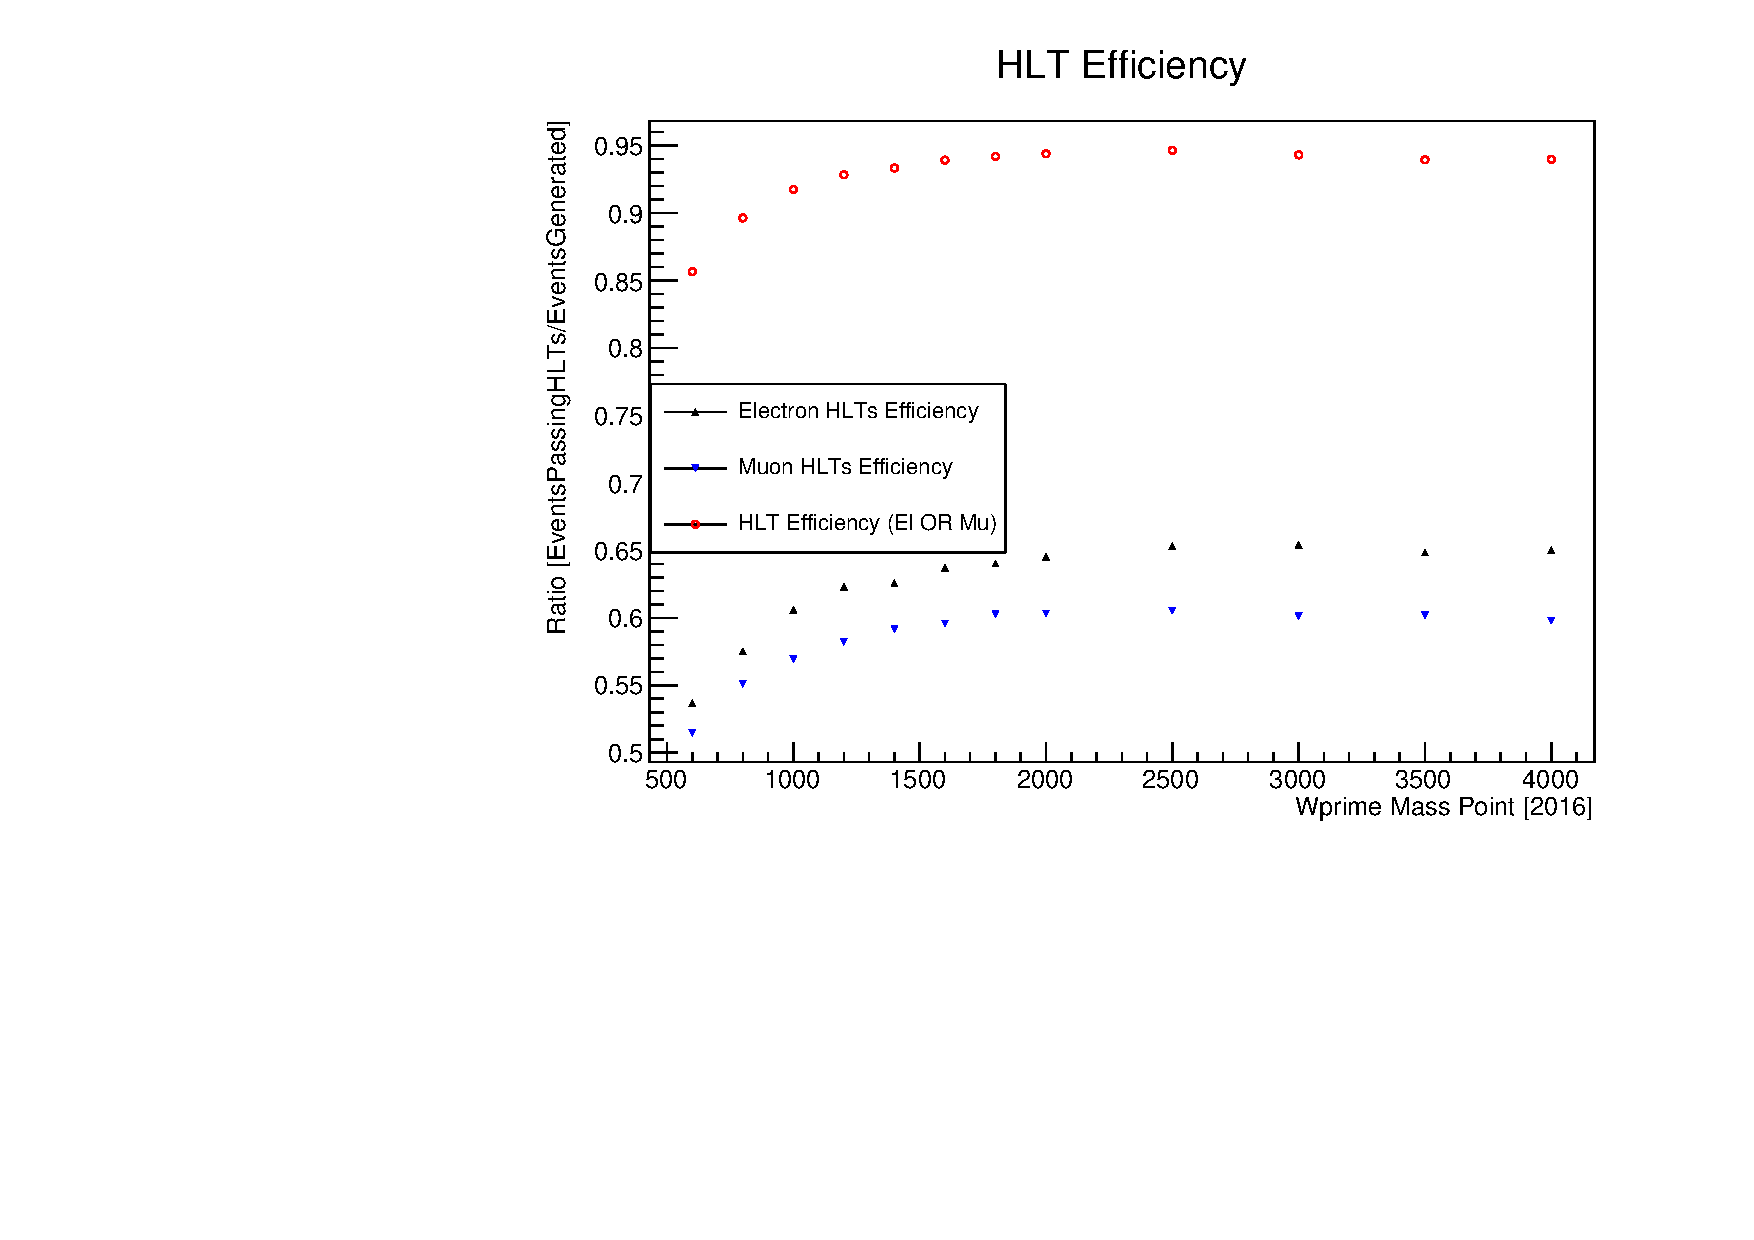
\includegraphics[width=.28\textwidth]{fig/2016_SignalTriggerEfficiency.pdf}}
        \subfigure[2017]{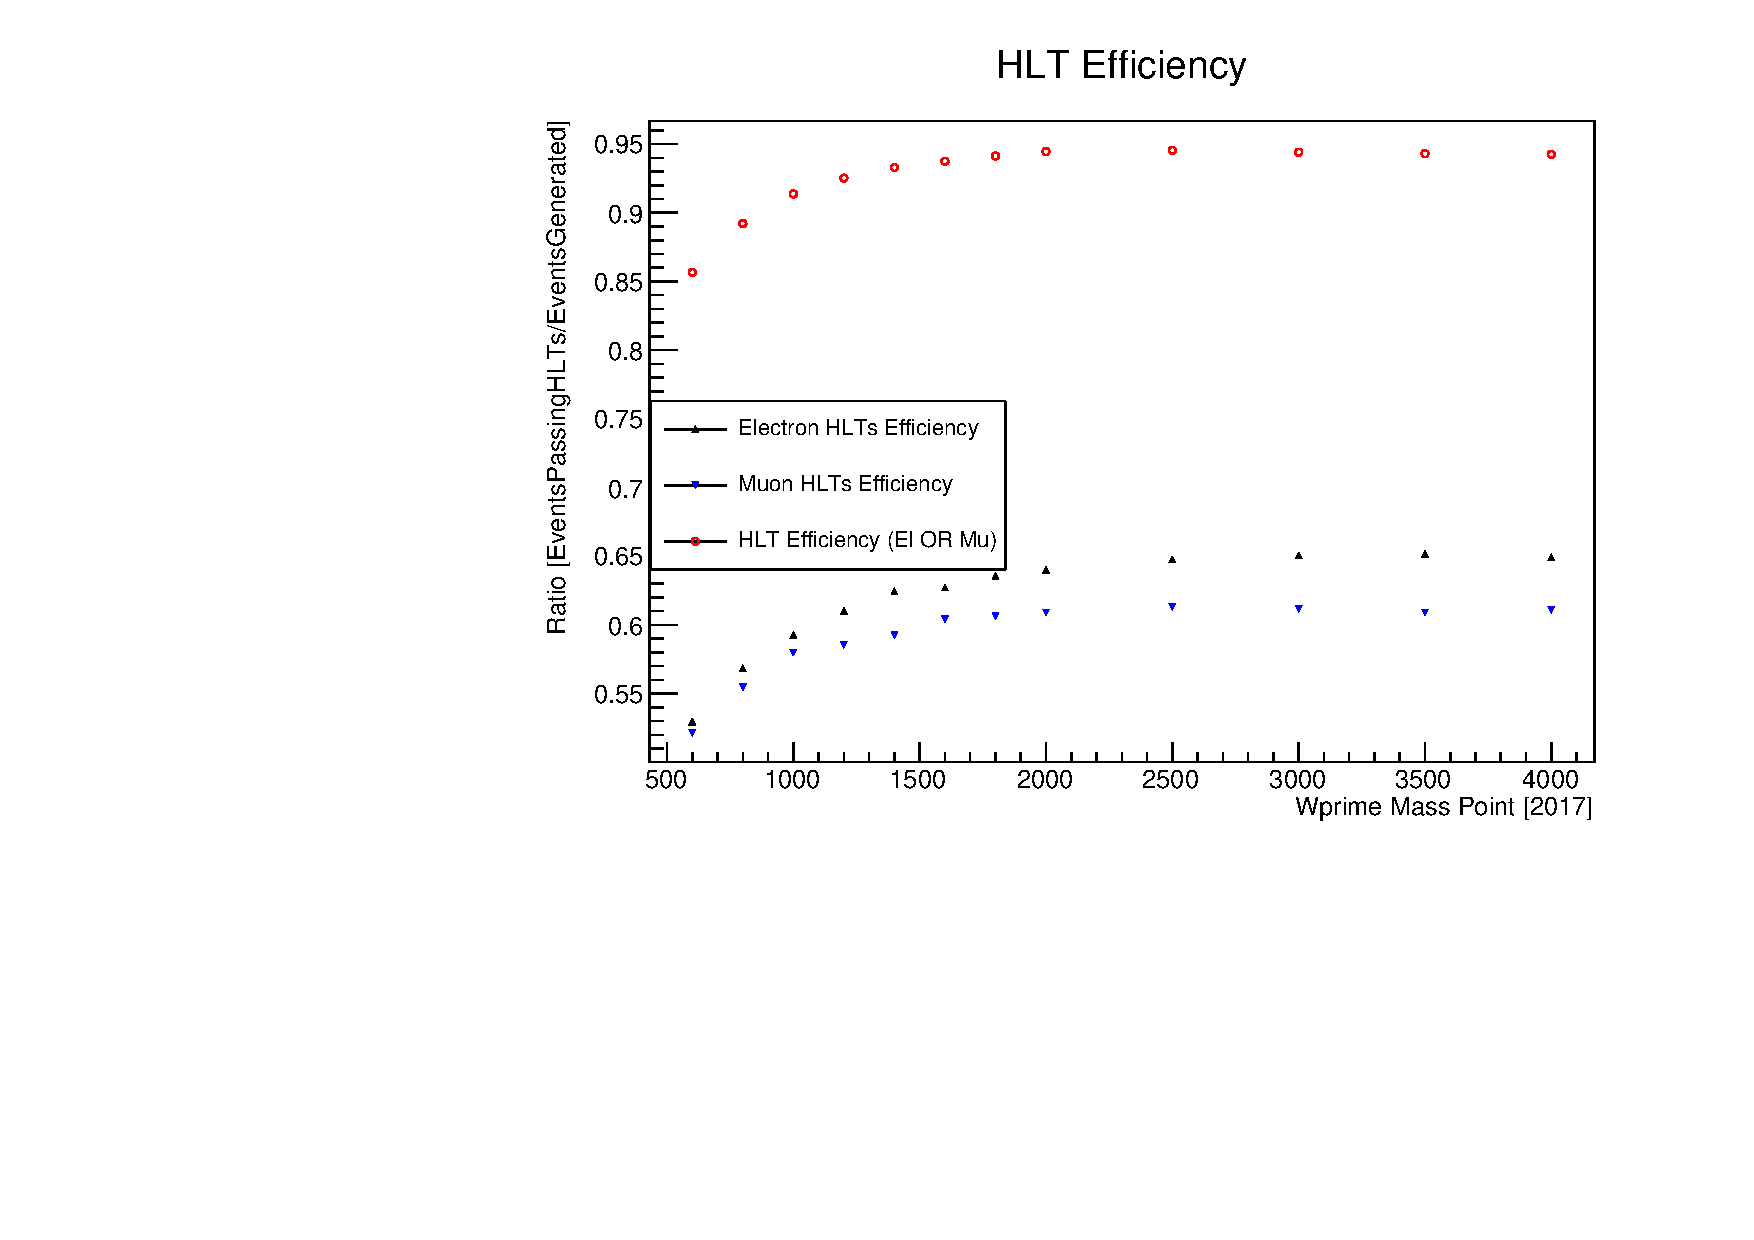
\includegraphics[width=.28\textwidth]{fig/2017_SignalTriggerEfficiency.pdf}}
        \subfigure[2018]{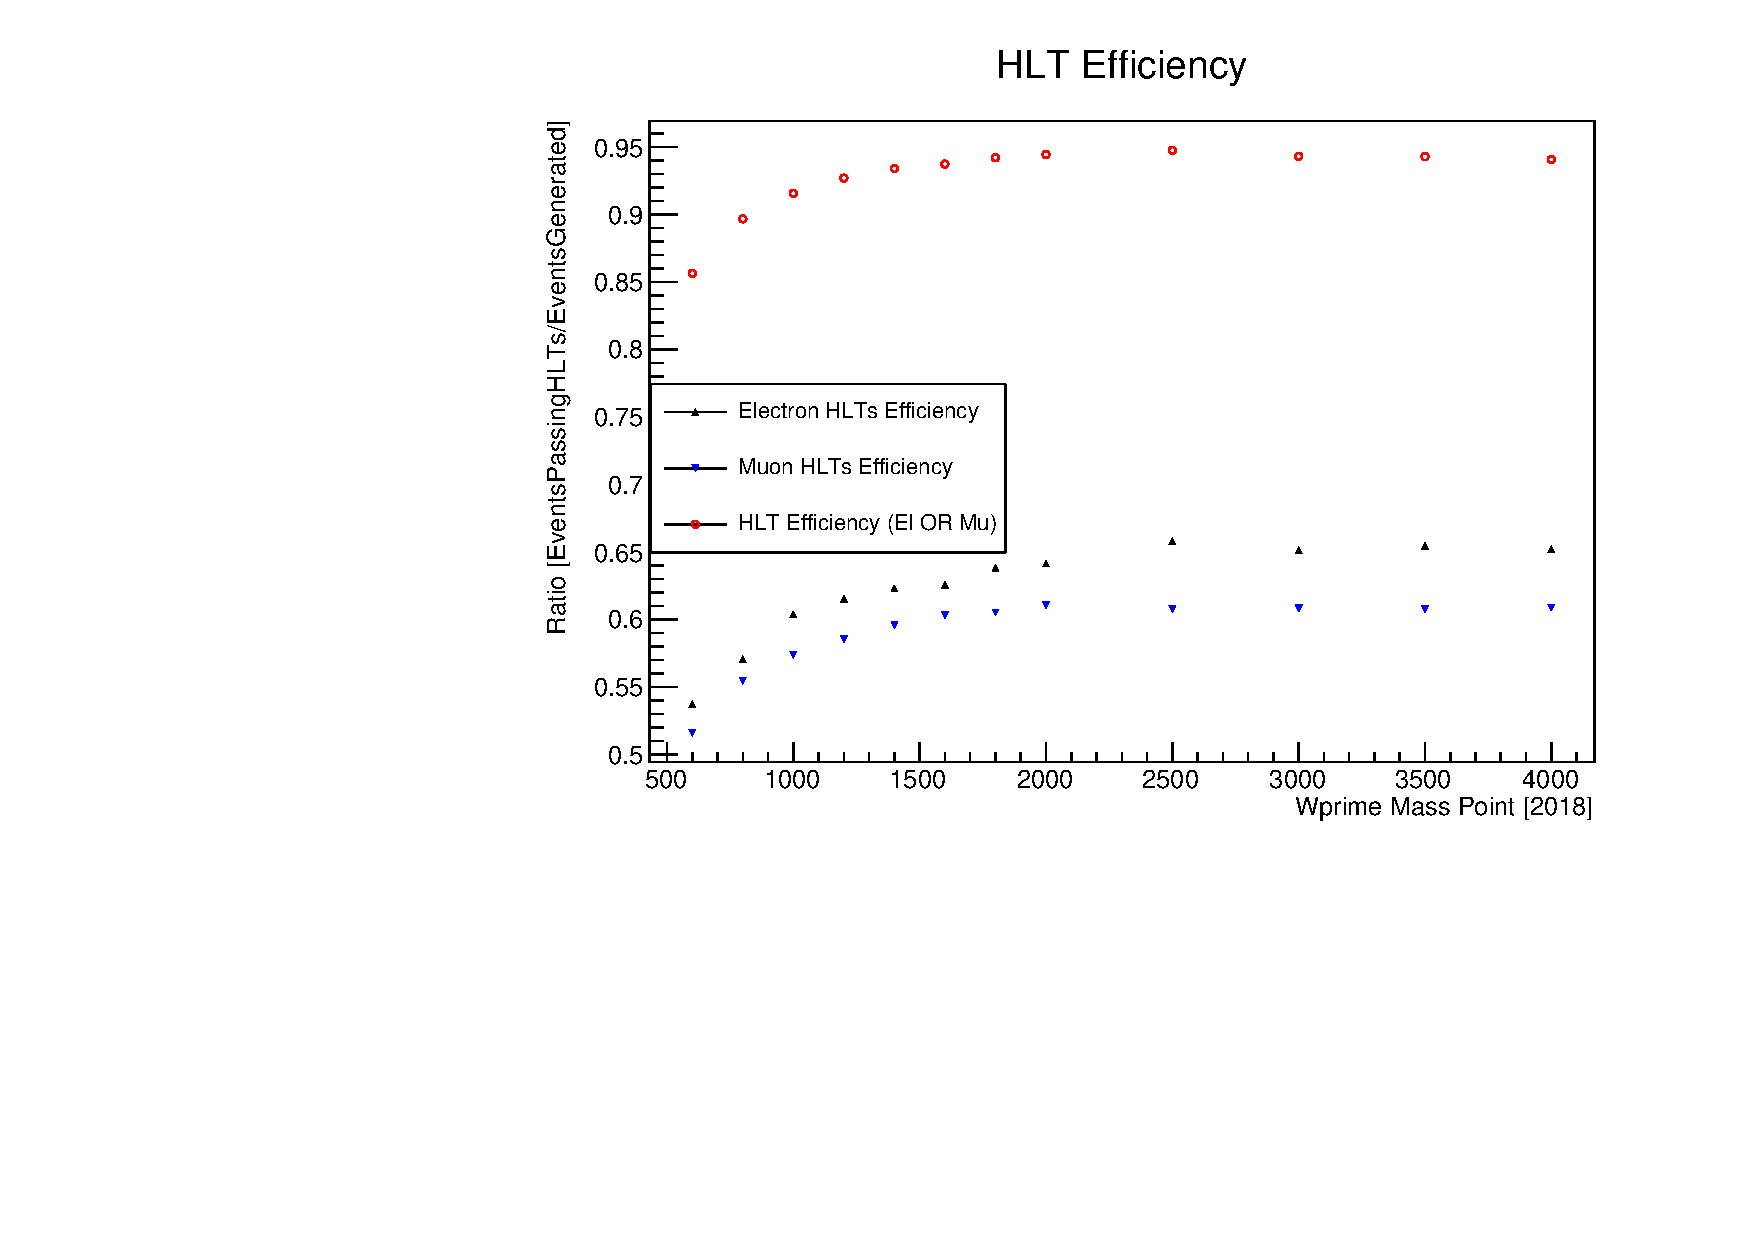
\includegraphics[width=.28\textwidth]{fig/2018_SignalTriggerEfficiency.pdf}}
  \caption{Signal efficiency for individual and combined High Level Triggers for Run II}
  \label{fig:hltSignalEfficiency}
\end{figure}

\begin{figure}[tph]
  \centering
  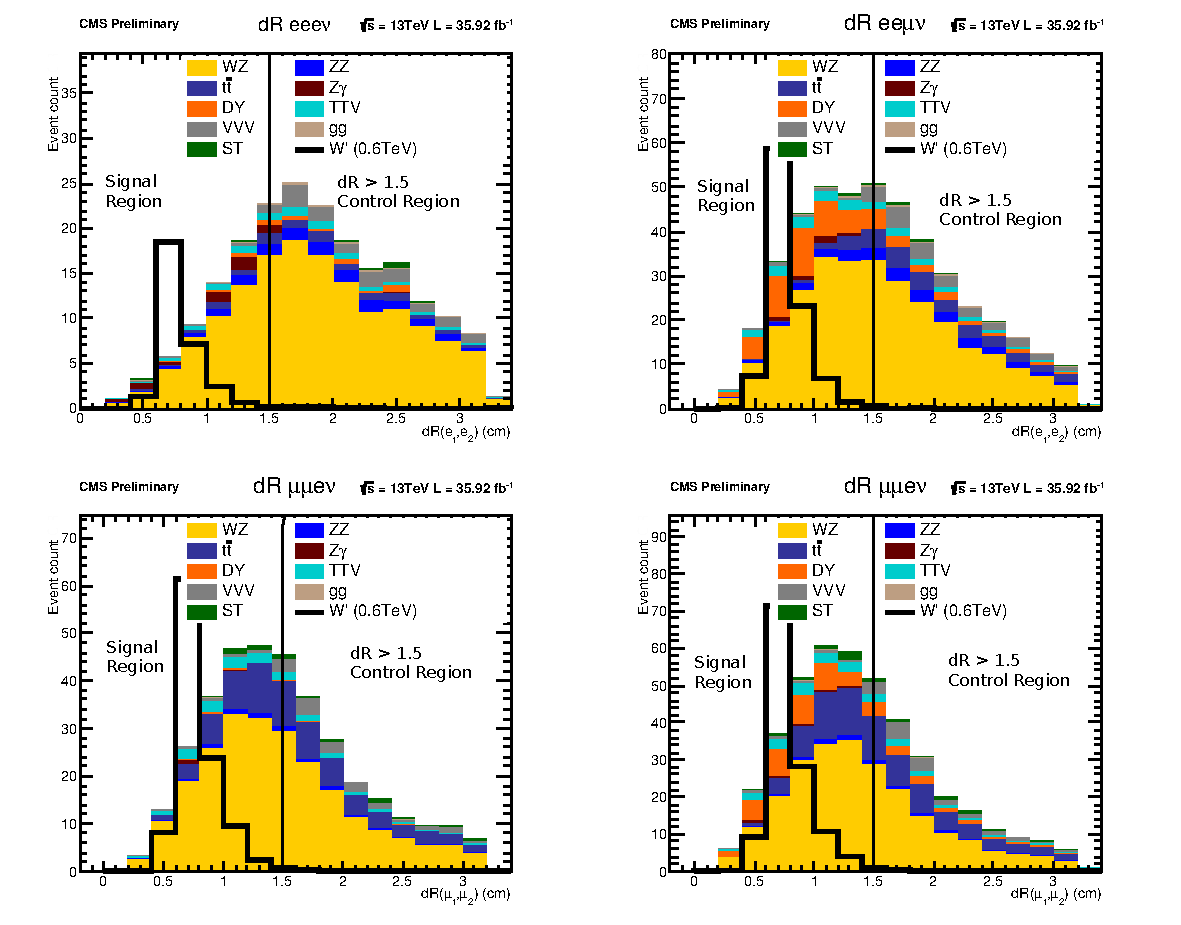
\includegraphics[width=\textwidth]{fig/Run2/KFactorIncluded_HDistl1l2_CR1_A+HDisM600.pdf}
  \caption{Definition of the signal and control regions. All the final signatures
    show how the region $dr_{l_{1}l_{2}} > 1.5$ is signal-depleted. A $600 GeV$
    mass resonance is used for illustration purposes. The larger the resonance
    mass, the narrower the signal distribution gets and it is shifted towards
    the lower $dR$ region as the leptons product of the $Z$ decay get closer
    forming a boosted topology.
    Top left: $Z(\rightarrow e+e)W(\rightarrow e+\nu)$
    Top right: $Z(\rightarrow e+e)W(\rightarrow \mu+\nu)$
    Bottom left: $Z(\rightarrow \mu+\mu)W(\rightarrow e+\nu)$
    Bottom right: $Z(\rightarrow \mu+\mu)W(\rightarrow \mu+\nu)$}
  \label{fig:ControlRegionDefinition}
\end{figure}

\begin{figure}[tph]
  \centering
  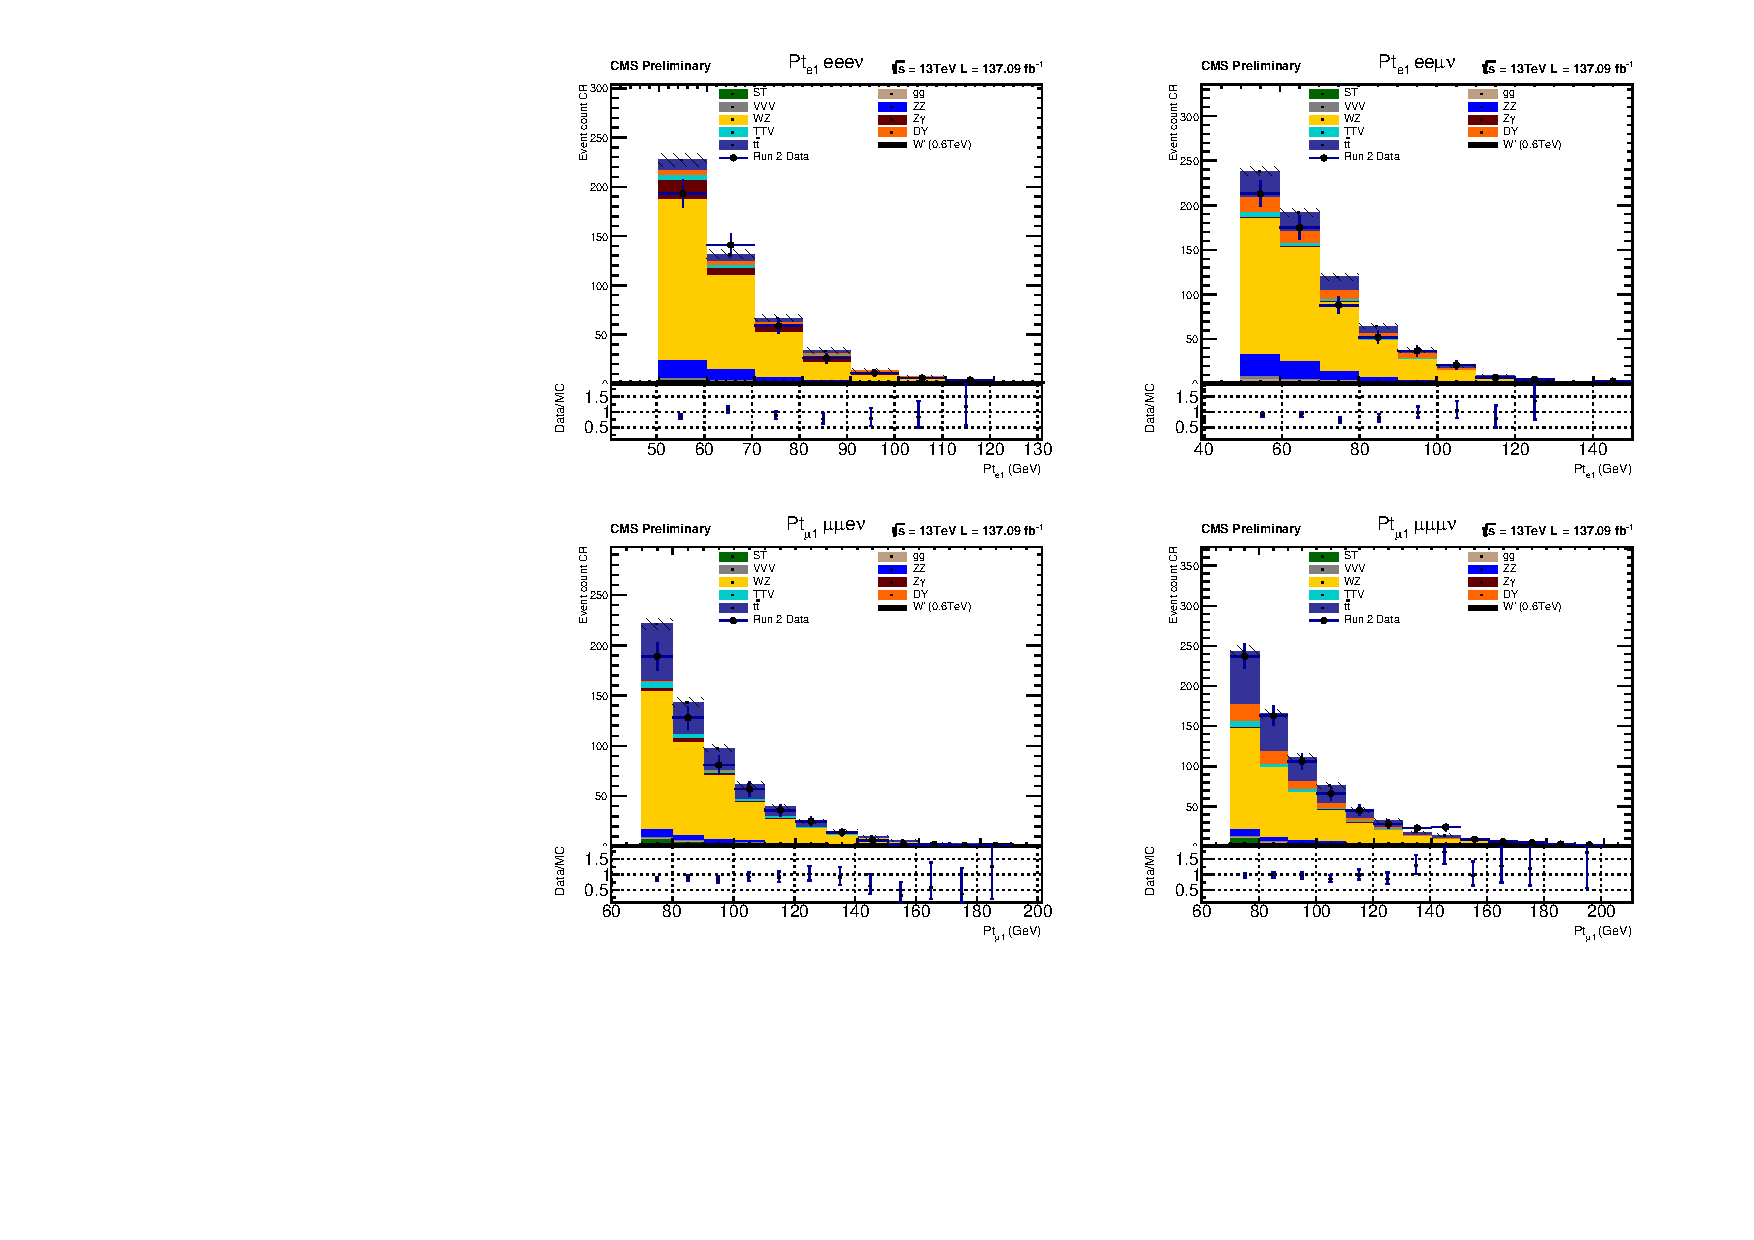
\includegraphics[width=\textwidth]{fig/Run2/KFactorIncluded_HPtl1_CR1_A_Run2_HPtRun2_M600.pdf}
  \caption{Leading lepton transverse momentum distributions for each final
    signature as seen in the $dr_{l_{1}l_{2}} > 1.5$ control region.
    Top left: $Z(\rightarrow e+e)W(\rightarrow e+\nu)$
    Top right: $Z(\rightarrow e+e)W(\rightarrow \mu+\nu)$
    Bottom left: $Z(\rightarrow \mu+\mu)W(\rightarrow e+\nu)$
    Bottom right: $Z(\rightarrow \mu+\mu)W(\rightarrow \mu+\nu)$}
  \label{fig:CR1_Run2_HPtl1}
\end{figure}

\begin{figure}[tph]
  \centering
  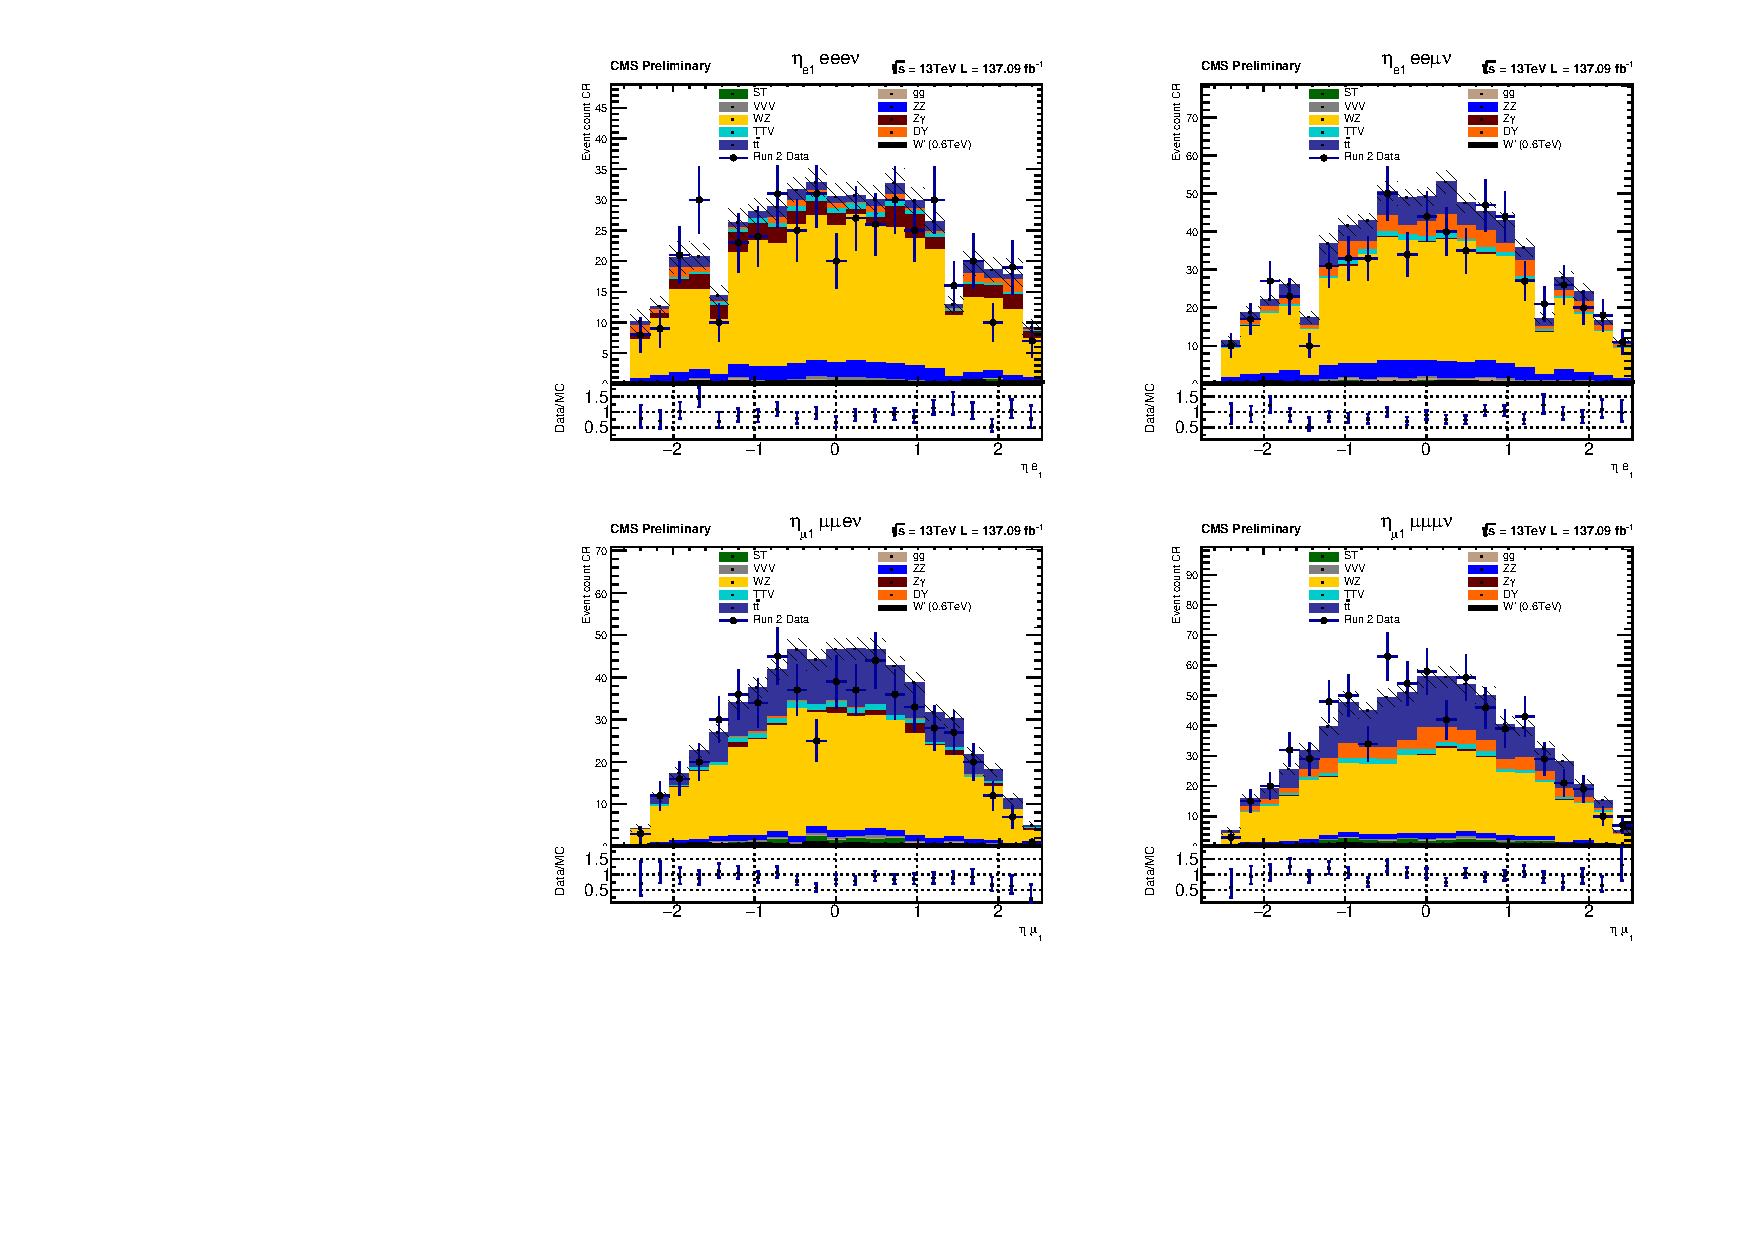
\includegraphics[width=\textwidth]{fig/Run2/KFactorIncluded_HEtal1_CR1_A_Run2_HERun2_M600.pdf}
  \caption{Leading lepton $\eta$ distributions for each final
    signature as seen in the $dr_{l_{1}l_{2}} > 1.5$ control region.
    Top left: $Z(\rightarrow e+e)W(\rightarrow e+\nu)$
    Top right: $Z(\rightarrow e+e)W(\rightarrow \mu+\nu)$
    Bottom left: $Z(\rightarrow \mu+\mu)W(\rightarrow e+\nu)$
    Bottom right: $Z(\rightarrow \mu+\mu)W(\rightarrow \mu+\nu)$}
  \label{fig:CR1_Run2_HEtal1}
\end{figure}

\begin{figure}[tph]
  \centering
  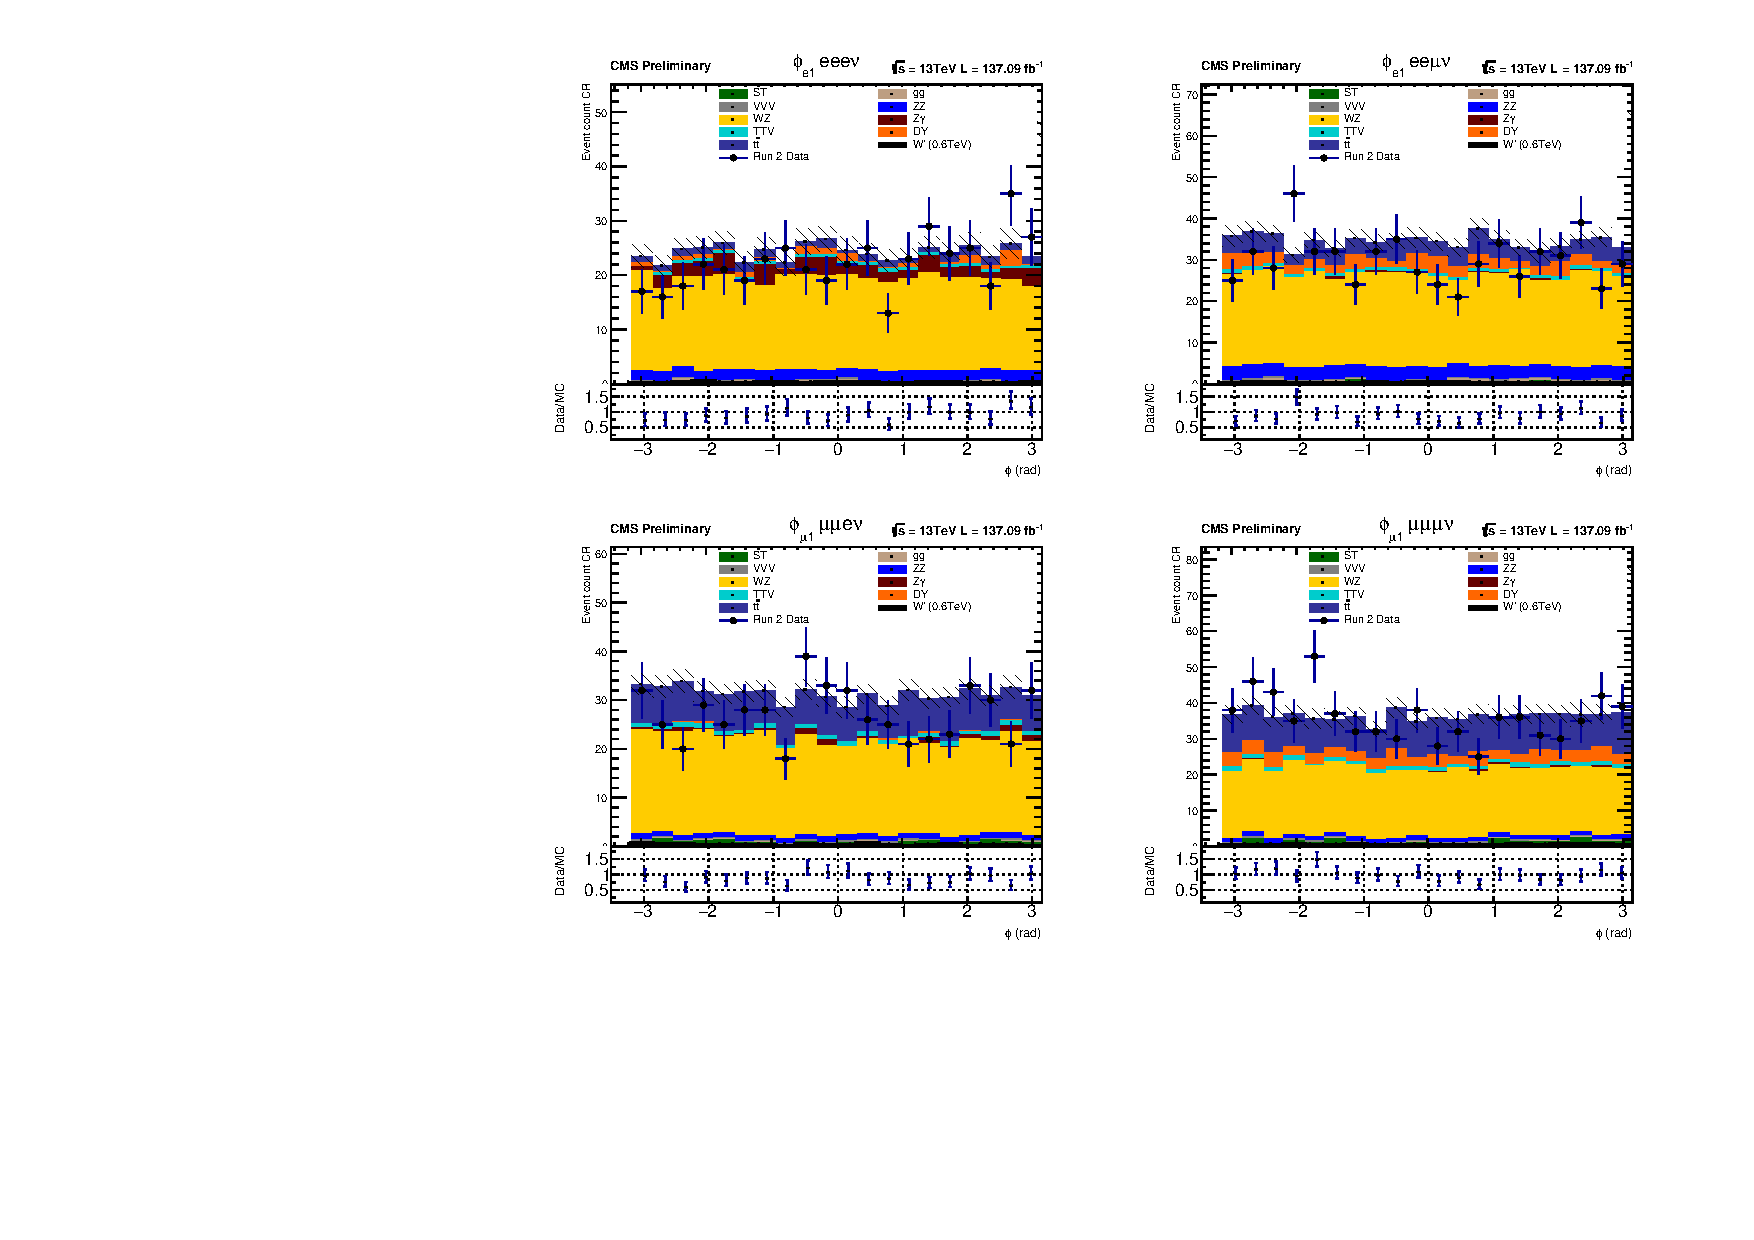
\includegraphics[width=\textwidth]{fig/Run2/KFactorIncluded_HPhil1_CR1_A_Run2_HPRun2_M600.pdf}
  \caption{Leading lepton $phi$ distributions for each final
    signature as seen in the $dr_{l_{1}l_{2}} > 1.5$ control region.
    Top left: $Z(\rightarrow e+e)W(\rightarrow e+\nu)$
    Top right: $Z(\rightarrow e+e)W(\rightarrow \mu+\nu)$
    Bottom left: $Z(\rightarrow \mu+\mu)W(\rightarrow e+\nu)$
    Bottom right: $Z(\rightarrow \mu+\mu)W(\rightarrow \mu+\nu)$}
  \label{fig:CR1_Run2_HPhil1}
\end{figure}

\begin{figure}[tph]
  \centering
  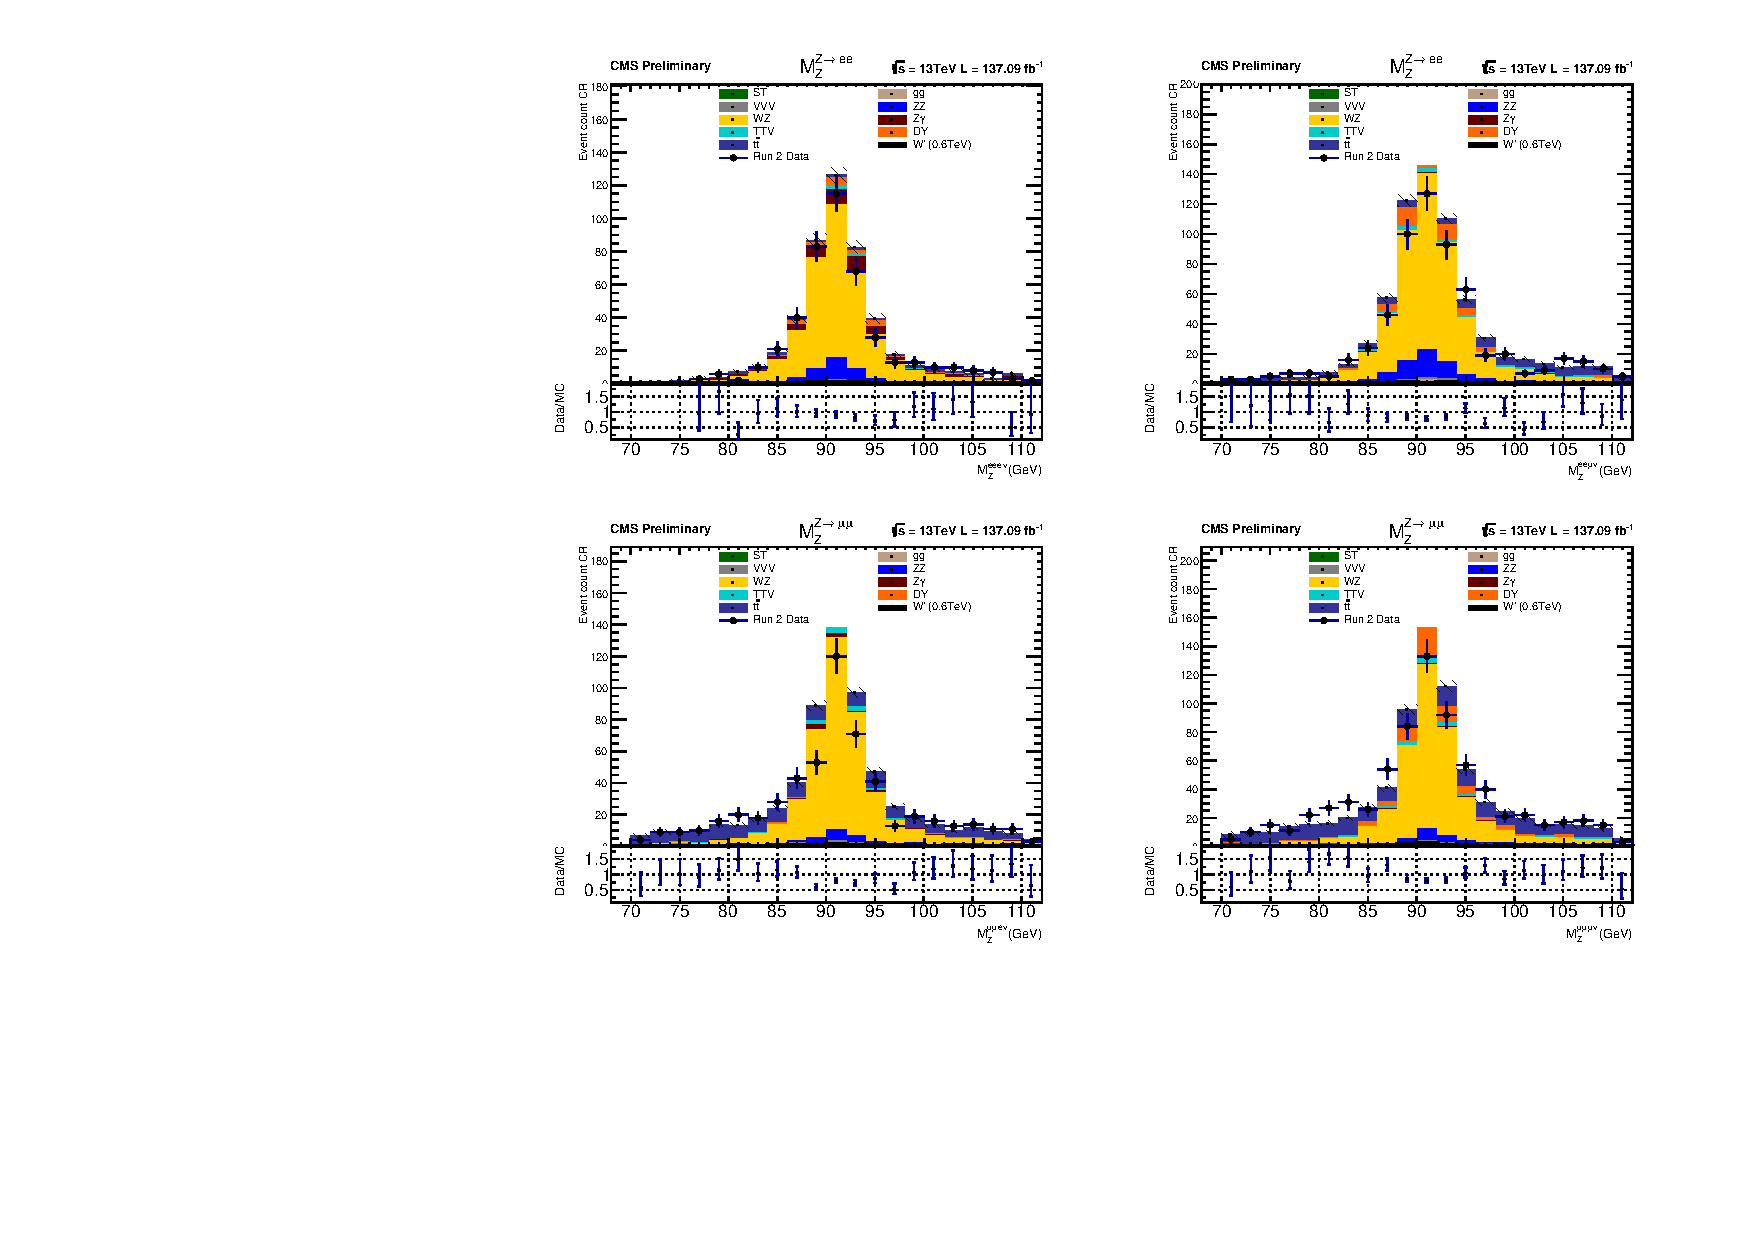
\includegraphics[width=\textwidth]{fig/Run2/KFactorIncluded_HMassZ_CR1_A_Run2_HMRun2_M600.pdf}
  \caption{$M_{Z}$ distributions of $Z\rightarrow\ell\ell$ candidates for each final
    signature as seen in the $dr_{l_{1}l_{2}} > 1.5$ control region.
    Top left: $Z(\rightarrow e+e)W(\rightarrow e+\nu)$
    Top right: $Z(\rightarrow e+e)W(\rightarrow \mu+\nu)$
    Bottom left: $Z(\rightarrow \mu+\mu)W(\rightarrow e+\nu)$
    Bottom right: $Z(\rightarrow \mu+\mu)W(\rightarrow \mu+\nu)$}
  \label{fig:CR1_Run2_HMassZ}
\end{figure}

\begin{figure}[tph]
  \centering
  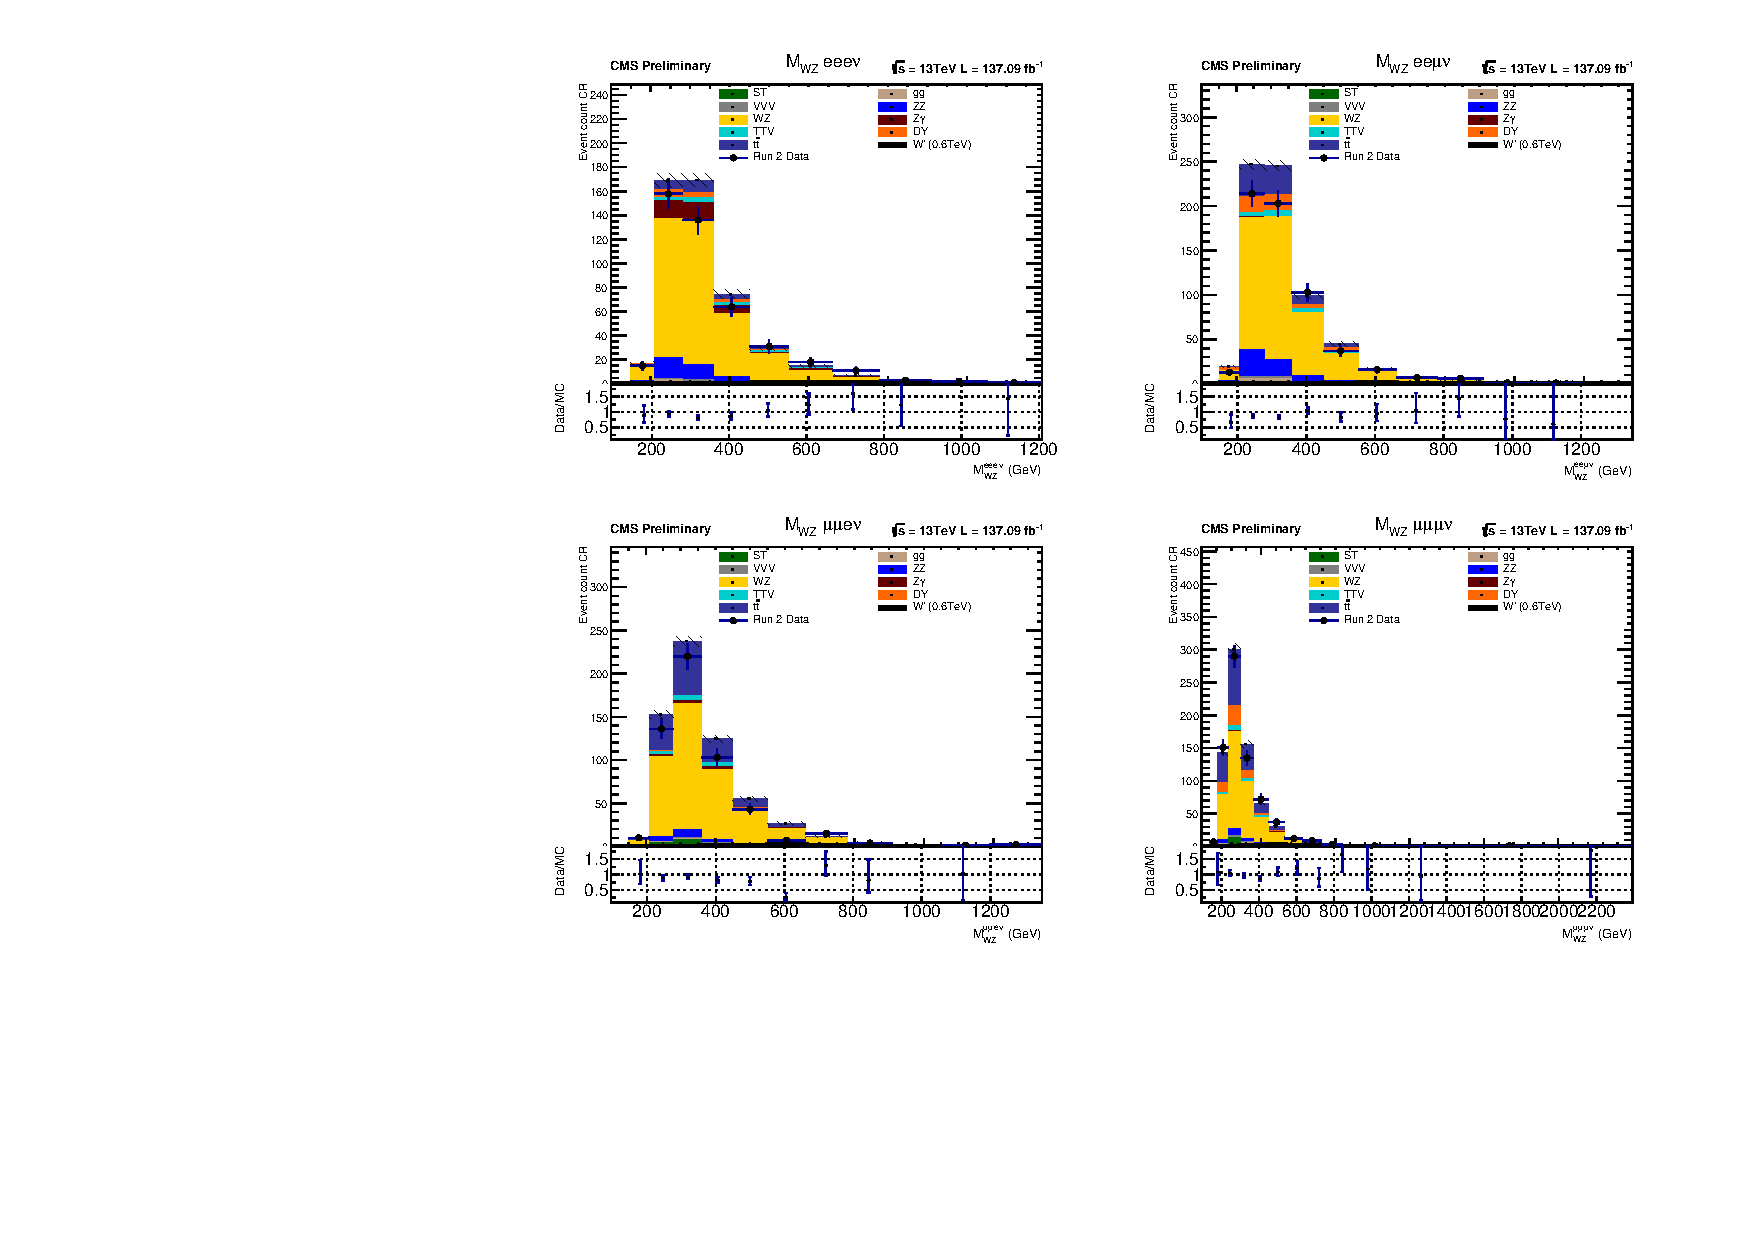
\includegraphics[width=\textwidth]{fig/Run2/KFactorIncluded_HMassWZ_CR1_A_Run2_HRun2_M600.pdf}
  \caption{The $WZ$ invariant mass after the $WZ$ candidate selection for each final
    signature as seen in the $dr_{l_{1}l_{2}} > 1.5$ control region.
    Top left: $Z(\rightarrow e+e)W(\rightarrow e+\nu)$
    Top right: $Z(\rightarrow e+e)W(\rightarrow \mu+\nu)$
    Bottom left: $Z(\rightarrow \mu+\mu)W(\rightarrow e+\nu)$
    Bottom right: $Z(\rightarrow \mu+\mu)W(\rightarrow \mu+\nu)$}
  \label{fig:CR1_Run2_HMassWZ}
\end{figure}

\begin{figure}[tph]
  \centering
  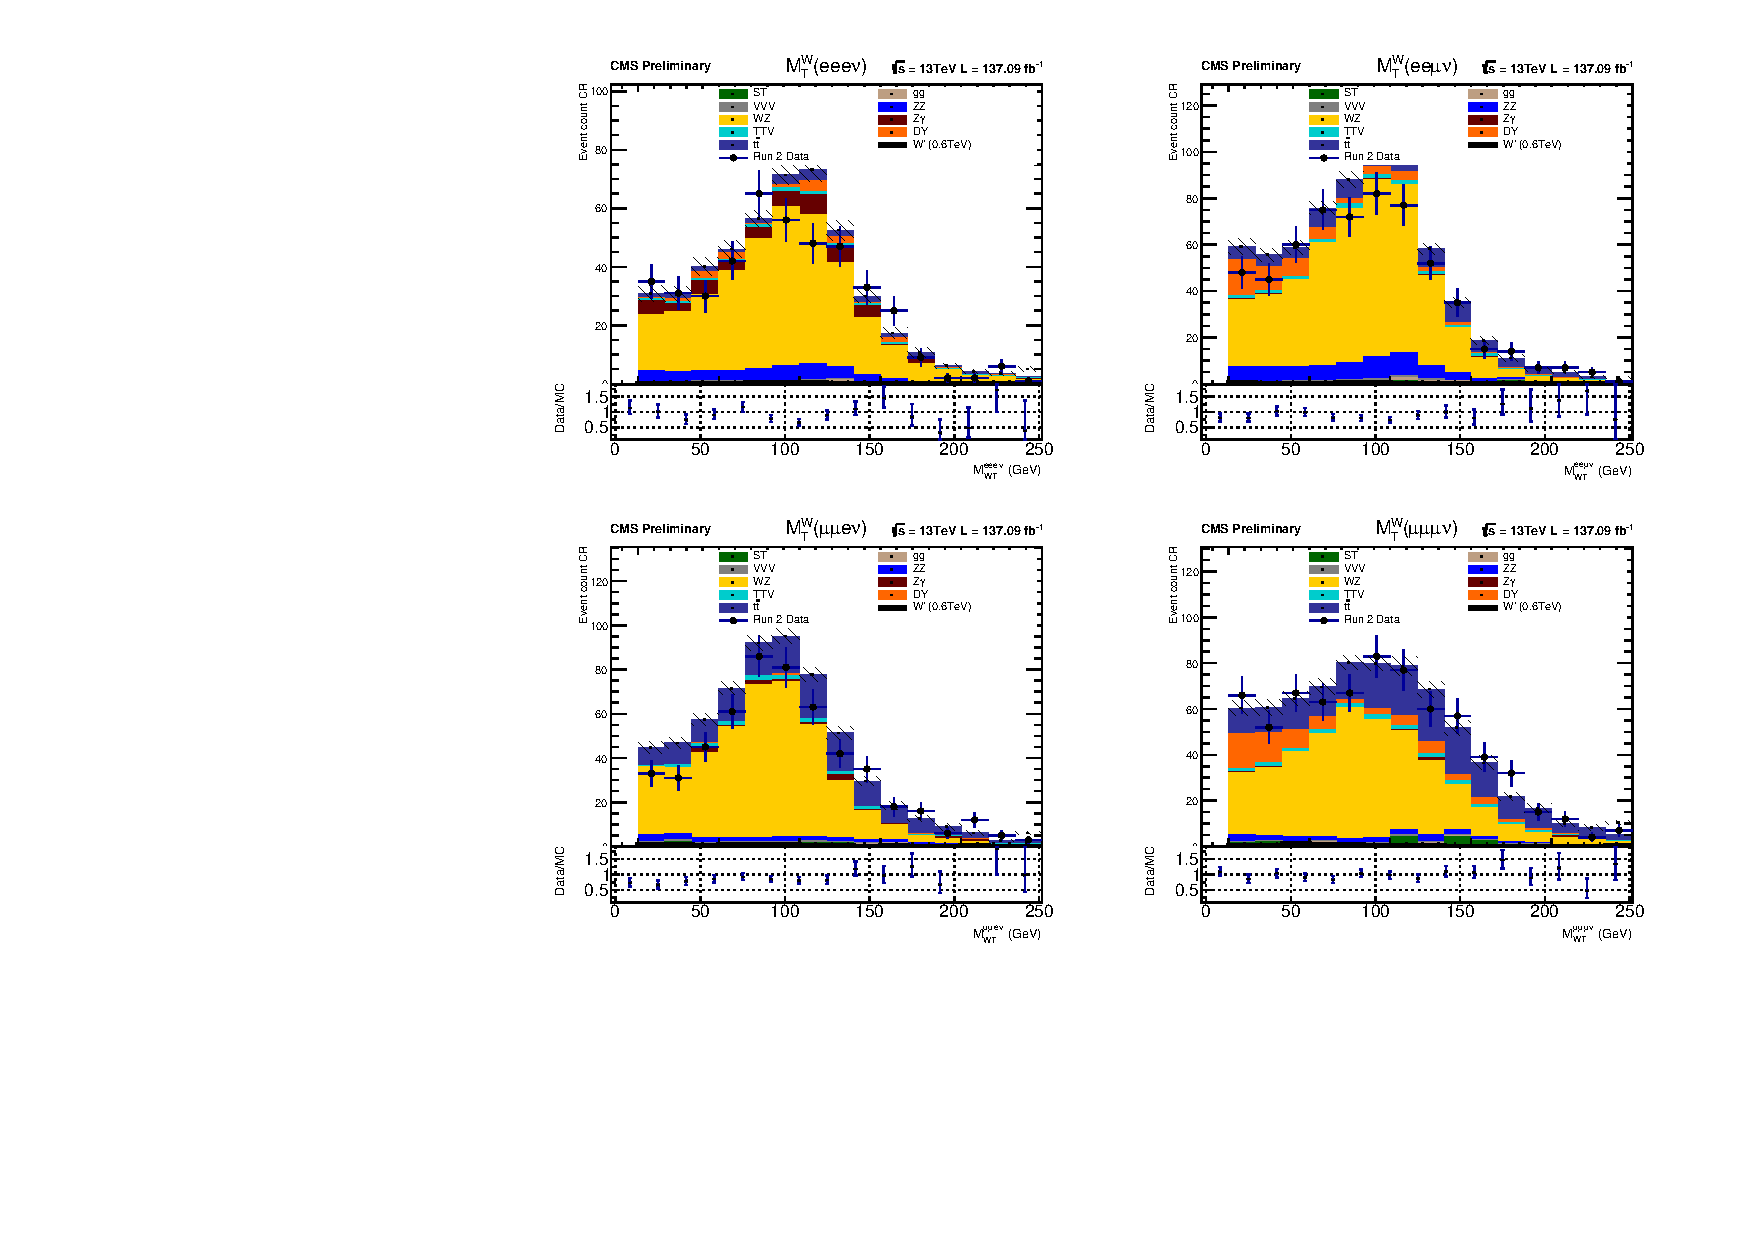
\includegraphics[width=\textwidth]{fig/Run2/KFactorIncluded_HMassTW_CR1_A_Run2_HRun2_M600.pdf}
  \caption{The transverse mass distribution for the $W$ candidate for each final
    signature as seen in the $dr_{l_{1}l_{2}} > 1.5$ control region.
    Top left: $Z(\rightarrow e+e)W(\rightarrow e+\nu)$
    Top right: $Z(\rightarrow e+e)W(\rightarrow \mu+\nu)$
    Bottom left: $Z(\rightarrow \mu+\mu)W(\rightarrow e+\nu)$
    Bottom right: $Z(\rightarrow \mu+\mu)W(\rightarrow \mu+\nu)$}
  \label{fig:CR1_Run2_HMassTW}
\end{figure}






